\documentclass[12pt, openany]{book}

\title{NeurExpo User Manual}
\author{Written by Eben Kadile & \newline & CATNIP Laboratory}
\date{}

\usepackage{natbib}
\usepackage{graphicx}
\usepackage{makeidx}
\usepackage{ifthen}
\usepackage[english]{babel}
\usepackage[utf8]{inputenc}
\usepackage{dirtytalk}
\usepackage{fancyhdr}
\usepackage{amsmath, amssymb, amsthm}
\usepackage{geometry}
\geometry{
  a4paper,
  total={8.5in,9.5in},
  top=1in,
  left=1in,
  right=1in
  }

\begin{document}

\pagestyle{fancy}
\fancyhf{}
\lhead{NeurExpo \thepage}
\rhead{CATNIP Laboratory}

\maketitle

\tableofcontents

\newpage

\section{Introduction}

NeurExpo is an application developed for the purpose of visualizing data recorded from neural populations in real-time. The application is written in \texttt{typescript} and is run in a web browser to maximize portability. The package downloadable from github has both the compiled \texttt{javascript} in \texttt{client/js} and the \texttt{typescript} source in \texttt{client/ts}.

The application is designed to receive data from a pre-processing server. That is, a server which performs spike-sorting as well as some additional dimensionality reduction algorithm such as online PCA, Kalman filtering, or Variational Joint Filtering.

An example \texttt{python} server which streams random data can be found in the \texttt{server} directory of the repo. There are two types of data to be visualized: the spikes of the individual neurons being recorded and the latent trajectory of the neural population (which may be higher than 3-dimensional).

The spike trains, which take the form of a sparse binary sequence, are rendered using a non-adaptive version of the \textit{gamma filter}, see section 4.1 or \cite{gammafilter}.

The latent trajectory is rendered using a method which allows the user to adjust which low-dimensional components of the data they are viewing.

Now I will give an in-depth tour of the GUI, explain how to transmit data from a server to the client, and describe the algorithms used to render each type of data.

\section{System Requirements}

The hardware requirements for the client will vary based on the dimensionality of the latent trajectory and the number of spike trains that are to be visualized. Any system with processors whose speed is at least 2 GHz and a graphics card should be absolutely fine. There is a setting which can make the graphics even less costly, so machines with integrated graphics should be able to render the visualization in real time as well.

The client system ought to have a web browser installed which is compatible with \texttt{websockets} and \texttt{WebGL} (most modern browsers satisfy this requirement).

In order to run the example \texttt{python} server, all that is required is \texttt{python} 2.7 or later and the `websockets` package.

\chapter{Initial Menu}

\begin{figure}
  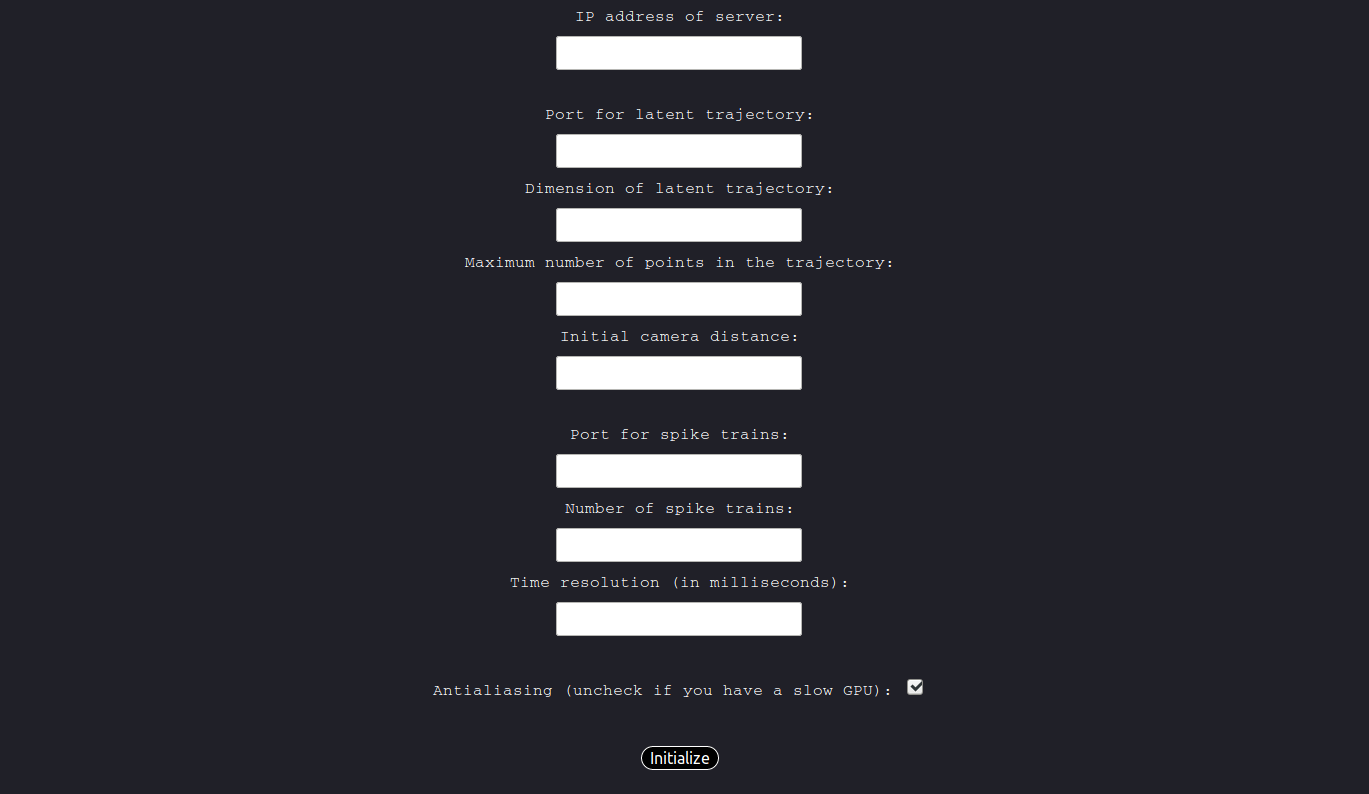
\includegraphics[width=\linewidth]{NeurExpo_Menu.png}
  \caption{The NeurExpo Initial Menu}
 \end{figure}

Upon opening \texttt{home.html}, found in the \texttt{client} folder, in your browser, you will be presented with a menu where you must input some information.

\section{IP Address}

The first piece of information is the IP address of the server which will be streaming the data. The server is assumed to be run by you or one of your collaborators, so it is up to you to obtain the IP address.

\section{Ports}

The second field is the port from which the latent trajectory will be streamed. The port from which our example \texttt{python} server streams the trajectory is \texttt{8200}. This can be changed in the \texttt{python} code, if you wish.

The sixth field is the port from which the spikes will be streamed. The port in the example server is \texttt{8400}. This can also be changed from the \texttt{python} code.

\section{Dimension}

The third field is the dimension of the latent trajectory. Once the transmission begins, the dimension will be sent to the server as a string with double quote characters at the beginning and end. This feature exists so that the server may adjust its inference algorithm to produce a trajectory of the desired dimension.

\section{Points on Trajectory}

The number of points on the trajectory determines how much history of the trajectory you will be able to view at once. A number between 100 and 500 is typically best for visualization. Entering a very large number may cause the visualization to lag.

\section{Camera Distance}

The distance from the camera to the origin can be adjusted during visualization using the scroll-wheel on your mouse. However, we must initialize this distance. The only way to appropriately initialize this distance is to know the approximate magnitude of the points which are being produced by the server's inference algorithm. Our example server produces points which typically have magnitude less than 1, so we can initialize the camera distance to 3.

\section{Number of Spike Trains}

This field simply corresponds to the number of spike train channels the server will be streaming. Once the transmission begins, this number is also sent to the server as a string with double quotes on both ends so that it can be compared to the number of spikes that the server was intending to receive. In the example server, the number of spike trains is simply this number which is received from the client.

\section{Time Resolution}

This field is in units of milliseconds, and tells you how history-sensitive the spike train rendering will be. If the number is too low, the spikes will fade too quickly to be seen. If the number is too high, old spikes will linger and it will become impossible to distinguish between neurons that are firing. Values will typically be between 10 and 100 milliseconds. If you expect the spike trains to be very sparse, the value should be higher; if you expect the firing rates to be high, the value should be lower. See the section on spike rendering for further details.

\section{Anti-aliasing}

Anti-aliasing refers to rendering a desired image multiple times with different offsets and then interpolating between the results so as to soften any pixelated edges that arise when the image is rendered only once. The render loop for \texttt{NeurExpo} is cheap, so most GPUs should be able to handle anti-aliasing. However, if you know you have a slow GPU, you may want to un-check \say{anti-aliasing}. This is a purely aesthetic feature; it will have no effect on the utility of the visualization.

\chapter{Rendering the Latent Trajectory}

\section{Covering the Grassmannian}

The fundamental challenge of rendering the latent trajectory is how to allow the user to view multiple 3-dimensional aspects of the high-dimensional data.

We solve this problem by allowing the user to adjust different sliders to view different low-dimensional components of the data, see Figure 2.1. More specifically, different configurations of the slider values correspond to different points on the Grassmannian: $Gr(3,n)$ where $n$ is the dimension of the trajectory. If you have little interest in the mathematics of the Grassmannian, you can still easily explore the low-dimensional components of your data by simply playing with the slider values.

\begin{figure}
    
\includegraphics[width=\linewidth]{latentLorenz.png}
    \caption{A 6-dimensional trajectory corresponding to a 3-dimensional Lorenz system. The Sliders below the Pause button will allow you to explore the different 3-dimensional projections of the trajectory.}
\end{figure}

The Grassmannian $Gr(k,n)$ is the topological space of k-dimensional linear subspaces of $\mathbb{R}^n$. This space has a manifold structure (indeed, it has a smooth structure as well), meaning some open sets of the Grassmannian can be parametrized by real numbers. We will focus on the Grassmannian $Gr(3,n)$, since this is what is relevant to our application.

We parametrize a relatively large open set of the $Gr(3,n)$ and then allow the user to adjust the real-valued parameters to determine which 3-plane the trajectory is projected onto.

Although some neighborhoods of the Grassmannian can be parametrized injectively, we sacrifice injectivity for the sake of covering a large portion of $Gr(3,n)$ in  a computationally efficient manner. Consider the subspace of $\mathbb{R}^n$, $V=span \{\boldsymbol{e}_1,\boldsymbol{e}_2,\boldsymbol{e}_3\}$ and a rank 3 linear map $T:V\rightarrow\mathbb{R}^n$. The reduced column eschelon form of the matrix representation of $T$ will be of the form

$$\begin{bmatrix} 1 & 0 & 0\\ 0 & 1 & 0 \\ 0 & 0 & 1 \\ a_{1,1} & \cdots & a_{1,3} \\ & \vdots & \\ a_{n-3,1} & \cdots & a_{n-3,3} \end{bmatrix}$$

$T$ specifies a 3D subspace of $\mathbb{R}^n$, and the values $a_{i,j}$ specify $T$. The orthographic projection matrix is computed by performing Gram-Schmidt orthonormalization on the columns of the above matrix and then taking the transpose. The orthonormalization is necessary to make sure that the trajectory isn't stretched or skewed after being multiplied by the projection.

If the set of values $a_{i,j}$ are related to another set of values $a'_{i,j}$ by an elementary row operation, then these two sets specify the same 3D subspace of $\mathbb{R}^n$. This introduces an unfortunate redundancy into our parametrization. However, if all $a_{i,j}$ were able to take any real value then the parametrization would be surjective, allowing the user to view the trajectory from any 3D subspace.

Naturally, it is impossible for \textit{all} real numbers to be represented on a computer. Instead we use exponential functions to make the sliders cover a very wide range of real numbers. Each slider takes values between $\pm 7\times 10^{106}$.

For more information on the Grassmannian refer to \cite{grassmannian}.

\section{Protocol for Transmitting the Trajectory}

The bytestring in each packet for the latent trajectory websocket is a sequence of 4-byte groups. The first group is a big endian unsigned integer which indicates how many trajectory points are encoded in the packet. Each 4-byte group after that is a 32-bit big endian floating point number corresponding to a coordinate of a point on the trajectory.

Thus, the dimension of the trajectory can be used to compute how many more 4-byte groups we expect after the group indicating the number of points. For example, if the trajectory is 12-dimensional and the first 4-bytes say that there are 3 points in the packet, then we expect that there are 36 more 4-byte groups in the packet, and that each group of 12 4-byte groups specifies a point in the trajectory.

\chapter{Rendering the Spike Trains}

\section{The Gamma Filter}

Suppose we have time-series data which takes the form of a sparse binary sequence called $s_t$ where $t\in\mathbb{N}$. We wish to construct a way to visualize this data such that we can observe multiple time-scales at once. Let $a$ be a real number. Then we can define the 4-layer gamma filter, $G_t^L$ by

$$G^1_{t+1}=aG^1_t+s_t$$
$$G^2_{t+1}=aG^2_t+G^1_t$$
$$G^3_{t+1}=aG^1_t+G^3_t$$
$$G^4_{t+1}=aG^1_t+G^4_t$$

Each layer follows an exponential decay until it is perturbed by the previous layer or the sequence $s_t$.

If $\Delta t$ is the amount of time between consecutive frames (about 0.15 milliseconds for most machines) then $a=2^{-h/\Delta t}$, where $h$ is the \say{time-resolution} (see section 2.7). This way, each layer follows an exponential decay with half-life $h$ when there is no input to the layer. See \cite{gammafilter} for more theoretical details on the gamma filter (note that that paper presents the gamma filter as an algorithm which \textit{learns} the optimal value for $a$, but we choose it before rendering).

Every spike train has its own gamma filter, but the value of $a$ is the same across all filters. Each filter is rendered as a set of concentric rings, with the inner disk representing $G^1$ and the outer ring representing $G^4$. See Figure 4.1.

\begin{figure}
    
\includegraphics[width=\linewidth]{spikes.png}
    \caption{Example frame of 32 spike trains being rendered.}
\end{figure}

\section{Protocol for Transmitting the Spike Trains}

Due to the nature of the gamma filter, the only data that is transmitted over the spike train websocket is the ID of the channel on which a spike is detected. This means that the client-side scripts do not detect latency in the connection. We have not noticed any performance issues while using a wireless connection. However, if low latency is absolutely critical then I recommend using an ethernet connection instead.

Specifically, every packet in this protocol is a sequence of 8-byte groups. The first four bytes of every group form a big endian unsigned integer indicating the ID of the channel from which a spike was detected. The second four bytes is a big endian unsigned integer which indicates how many spikes were detected on the given channel since the last packet was sent. Since your server can most likely send packets faster than a neuron can fire, this number is almost always 1.

\chapter{Using the Example Servers}

Included in the NeurExpo repo is python code for a pair of example servers. These two scripts were written to provide an accessible illustration of how to use the spike and trajectory transmission protocols.

With python 2.7 or later and the python `websockets` package installed, simply run both of these scripts on separate command lines. You will be asked to input the desired ports, the dimension of the trajectory, and the number of spike trains. After inputting this information, the servers will wait for a request from the client. Enter the corresponding information into the client's menu, and initialize. The trajectory server will send a noisy Lorenz system over the websocket, and the spike train server will send a procedural spike train.


\chapter{Navigating the GUI}

Here we provide a simple walk-through of \texttt{NeurExpo}'s graphical user interface.

After you've entered the necessary information in the initial menu, clicking \say{Initialize} will allow the system to store the information you entered and re-write the \texttt{html} document.

At this stage you may want to check that there were no parse errors in the information that you entered in the menu. Depending on your browser, you can do this by right clicking the window, clicking \say{Inspect Element}, then clicking \say{Console}; any errors should be printed here.

If there do not appear to be any errors, clicking \say{Begin Transmission} will open two websockets to the server: one for the latent trajectory and one for the spike trains. The system will immediately send the server trajectory dimension that it is expecting and the number of spike trains that it is expecting (it is critical that the server and client agree on dimension and number of spike channels). The client will render data as soon as it starts receiving it from the server.

The latent trajectory will be rendered on top. If the trajectory is 3D or higher, you can click and drag on the canvas to rotate the camera as well as hover your cursor on the canvas and use your scroll-wheel to zoom in and out.

The spikes will be rendered on the lower canvas. If there are a lot of them, you may have to scroll down on the page to see them all.

The \say{Pause} button will stop the render loop, but it will not close the websockets or pause the gamma filter. The \say{End Transmission} button will close the websockets.

\bibliographystyle{plain}
\bibliography{references}
\end{document}
